\documentclass{article}

\usepackage[utf8]{inputenc}

% Packages
\usepackage{amsmath,amssymb}
\usepackage{bm}% boldmath
\usepackage{listings} % Code block (source code) \begin{lstlisting} 
\usepackage{natbib}
\usepackage{graphicx}
\usepackage{lmodern}
\usepackage[usenames,dvipsnames,svgnames,table]{xcolor}
\usepackage[textwidth=16cm,textheight=23cm]{geometry}

%\usepackage{inconsolata} % New monospace font

% URL
\usepackage{url}
\usepackage[colorlinks=true, a4paper=true, pdfstartview=FitV, linkcolor=blue, citecolor=blue, urlcolor=blue]{hyperref}

% Figures
\usepackage[font=small, labelfont=bf]{caption}
\usepackage{subfig} % Subfigures. Uses \subfloat[captions text]{figure}

% Tables
\usepackage{booktabs}   % Allows the use of \toprule, \midrule and \bottomrule in tables for horizontal lines
\newcommand{\ra}[1]{\renewcommand{\arraystretch}{#1}} % spaces in tables

% Itemize
\usepackage{enumitem}

% Commands
%\newcommand{\code}[1]{\texttt{#1}} % \code{inline code}
\newcommand{\code}[1]{{\small\ttfamily #1}} % \code{inline code}
\newcommand{\expval}[1]{\langle #1 \rangle} %
\renewcommand{\theequation}{\arabic{section}.\arabic{equation}} % Book format equation
\renewcommand{\thefigure}{\arabic{section}.\arabic{figure}} % Book format figure
\renewcommand{\vec}[1]{{\bf #1}} % Lars likes this better than arrow

% Set page attribution
\setlength{\parindent}{0pt}


% PSTRICKS
\usepackage{pstricks,pst-node,pst-tree} % includes graph additions
\usepackage{pst-pdf} % Compiles the pictures
\usepackage{pst-node}
\usepackage{pst-plot}
\usepackage{pst-3dplot}
%\usepackage{pstricks-add,babel}


\definecolor{lbcolor}{rgb}{0.9,0.9,0.9}  

\lstset{
language=Python,                        % Code langugage
commentstyle=\color{gray},              % Comments font
basicstyle=\small\ttfamily,             % Code font, Examples: \footnotesize, \ttfamily
keywordstyle=\bfseries\color{blue},
stringstyle=\color{orange},
numbers=left,                           % Line nums position
numberstyle=\tiny,                      % Line-numbers fonts
stepnumber=1,                           % Step between two line-numbers
numbersep=5pt,                          % How far are line-numbers from code
frame=none,                             % A frame around the code
tabsize=4,                              % Default tab size
captionpos=b,                           % Caption-position = bottom
breaklines=true,                        % Automatic line breaking?
breakatwhitespace=false,                % Automatic breaks only at whitespace?
showspaces=false,                       % Dont make spaces visible
showstringspaces=false,                 % Dont make spaces visible in strings
showtabs=false,                         % Dont make tabls visible
belowskip=8pt,
morekeywords={range, xrange, as},
backgroundcolor=\color{lbcolor},  
showstringspaces=false
% emph={[2]root,base}
% morekeywords={one,two,three,four,five,six,seven,eight,
}


%commentstyle=\color{gray},              % Comments font
%basicstyle=\small,                      % Code font, Examples: \footnotesize, \ttfamily



%basicstyle=\footnotesize\ttfamily,
%keywordstyle=\bfseries\color{green!40!black},
%commentstyle=\itshape\color{purple!40!black},
%identifierstyle=\color{blue},
%stringstyle=\color{orange},







% ***************************************************
% HEADER INFORMATION

\title{Exercise 1}
\author{Molecular Statistics, Week 1}
\date{}

% ***************************************************

\begin{document}


% ***************************************************
% BEGIN DOCUMENT
% ***************************************************

\maketitle

\section*{Introduction}

The exercises are split into two parts: A general introduction to new concepts and programming tricks and the main part which is to simulate physical systems.
It is very important that you go trough each exercise, type each example code in exactly and run it.
That means, \textsc{do not copy-paste}.
The point of the exercises is to train in how to write, read and debug code - the more work you put into getting the basics down the easier it will be to solve future exercises.\\


There is no Python curriculum, but two online books, namely
\href{http://learnpythonthehardway.org/book/}{learnpythonthehardway.org/book} and
\href{http://pymbook.readthedocs.org/en/latest/}{pymbook.readthedocs.org/en/latest},
contains all the concepts with examples.
However, this being a programming course we require you to use Google for most information searching and debugging.

\section{Python Introduction}

First thing first, we want to create our very first program.
To run programs with python we save a file with the extension \code{.py} and run it via the terminal window.
Write the following python code and save it as \code{example\_program.py}

\begin{lstlisting}
# you can use comments underway to remind yourself later what the code should do
print "I want to print this statement" # you can also comment after a line
\end{lstlisting}

run it as

\begin{lstlisting}
python example_program.py
\end{lstlisting}

Is the output as expected?
%
Now, let's start by getting to know Python better - starting with some simple examples. Remember to use the \code{print} statement in your program to print the result of the following examples.
We encourage you to have some sort of logical file system, saving all the exercises in different files and folders so you can find it again when needed. \\

Some useful commands for navigating your file system can be found in the folder \textbf{Guides} on Absalon.  The document is called \textbf{Terminal Guide}.
Download it and keep it as reference for when working with the terminal\footnote{Do take a look at the other guides as well}.\\

\subsection{Introduction to Python}

Now, imaging that you are planning to bake a cake for the next exercise-class in molstat.
Before you go to the shop you want to know how much money  to bring.
You look up a recipe and see that you need to buy:

\vspace{10pt }
 
\begin{center}
    \begin{tabular}{c r r r}
    \hline
    Ingredient & Price & Units/Pcs needed & Unit weight \\
    \hline
    Flour & 8 kr. & 1  & 2 kg \\
    Eggs & 28 kr. & 1  & 10 pcs \\
    apple & 2 kr./pcs & 5   & N/A\\
    Sugar & 10 kr.& 1  & 1 kg \\
    Icing sugar &  8 kr. & 1   & 0.5 kg \\
    Butter & 16 kr. & 1  & 200 g \\
    \end{tabular}
\end{center}

First you need to find out how much money to bring to the shop.
Python can do this for you by working as a simple calculator.

\begin{enumerate}
    \item Execute the following statements.
\begin{lstlisting}
print 2+3
print 2.0*3.0+4.0
print 5*6
print 5.0*6.0
print 28/10
print 28.0/10.0
\end{lstlisting}
    Does Python behave like your regular calculator?
    {\em Hint}; what is the difference between {\code{integer}} and {\code{ float}}? 
    
    \item Use Python  to calculate the total price of the items on you shopping list  
\end{enumerate}

Once you've added up the total amount you realise that it might be cheaper to buy a cake instead.
In order to check that you must calculate the actual price of the cake you are making.
In order to bake the cake you need:

\begin{center}
    \begin{tabular}{c l l}
    \hline
    Ingredient & Amount needed\\
    \hline
    Flour & 175 g \\
    Eggs & 1 pcs \\
    Apple & 5 pcs \\
    Sugar & 100 g \\
    Icing sugar &  20 g \\
    Butter & 75 g \\
    \end{tabular}
\end{center}

\begin{enumerate}[resume]

    \item Use Pyhton to calculate the total price of your cake.
 
\end{enumerate}

% NOTE: Python also knows the more advanced functions found on a calculator. Try the following.
% \code{5**2, 5\%2} and explain the output.\\

Manually entering numbers really does us no good, we might as well use a calculator.
Instead, we want to utilize what programming languages can provide,
namely storage of values in what is known as {\bf variables}.
Variables can store anything that you can think of, i.e. integers, floats, strings, lists so forth.
Variables are assigned values by specifying a variable name and a value, e.g.

\begin{lstlisting}
variable_name = 5.0
\end{lstlisting}

where a variable named \code{variable\_name} has been assigned the value
of $5.0$.
Some restrictions apply for variable names (must start with a letter, can't have names of in-build functions etc.), but otherwise we are not restricted in the naming.\\

Give your {\bf variables} useful names, such as \code{no\_particles} for representing number of particles.
That way you can easily remember what values are stored in the variable and it makes the code more readable for others.

\begin{enumerate}[resume]
    \item Make 6 {\bf variables}, one for each ingredient, and assign a value equal to the price pr. g/pcs. e.g 
    \code{flour\_price\_pr\_g = 8.0/(2*10**3)}
    \item Use these variables to calculate the total price of the cake, and store the total price in the variable \code{price}.
    \item Print the total price of the cake
    \item Why would it be a good idea to calculate the total price with variables instead?
\end{enumerate}

On the same note, it is always a good idea to leave short comments in your program to remind yourself/ explain to others what each little section of code is used for.
Commenting is done by starting the line with \#.

Since a variable can contain anything, a very useful function is \code{type(arg)}, where \code{arg} is a variable.
This function will return the type of value stored in the variable.\\

In this way you could calculate the price of the cake when shopping in different stores simply but changing the variable containing the price pr. gram of the ingredients. \\

Usually when working with a program we work with a range of numbers that we need to manipulate, and for this it is fairly useful to create a Python {\bf list} of numbers.
A list is defined with the same syntax as a float variable;

\begin{lstlisting}
prices_list = []
\end{lstlisting}

The above code creates an empty list named \code{prices\_list}.
Even though the list is empty we can still print the content of the variable (try it).
If you want to add an element to the list you can append it using \code{list\_name.append(arg)} where \code{arg} is the element to be appended to the list.

For example if you want to append 2.0 to a list you write;

\begin{lstlisting}
prices_list.append(2.0)
\end{lstlisting}

or if you want to append the value of a variable

\begin{lstlisting}
prices_list.append(flour_price_pr_g)
\end{lstlisting}

\begin{enumerate}[resume]
    \item Create an empty list called \code{price\_list}.
    Print the empty list.
    Append \code{flour\_price\_pr\_g} and print the list again.
    What changed in the output?

    \item Print the type of the variable.

 \end{enumerate}


Different variables have different attributes, which are called {\em methods}.
These methods are executed using 'dot'.
For instance, the variable of type list has the method \code{sort()}, which can be called as follows;

\begin{lstlisting}
prices_list.sort()
\end{lstlisting}

For a list of floats, this results in the items of the list being sorted by value.\\

Another way of populating a list with numbers is to do it directly when we create the list.
This is done almost the same way as when we created the empty list, except we
provide the initial content right away. E.g.

\begin{lstlisting}
another_price_list = [1.0, 2.0, 3.0, 4.0, -2.0, -4.5, -1.0]
\end{lstlisting}

\begin{enumerate}[resume]
    \item Create \code{another\_price\_list} with the prices of you ingredients like in the above example.\\
    Print \code{another\_price\_list}. Sort the list. Print the sorted list. \\
    Does it provide the correct result?

    \item Print \code{another\_price\_list} in reverse sorted order.
    Use Google to find out how.\footnote{Using Google is
    by far the most important tool as a programmer.}
\end{enumerate}

% >>> L = [0,10,20,40]
% >>> L.reverse()

If we want to access the i'th element in a list
we use square brackets. To print the \textbf{second element}
in \code{another\_price\_list} you write;

\begin{lstlisting}
print another_price_list[1]
\end{lstlisting}

Notice that we wrote 1 and not 2. This was not a typo!
This is because the {\bf{list index starts at 0 and not 1}}.\\

To get the length of a list you use the function \code{len(arg)}
where \code{arg} is the variable with the list.
If you want the length of our example list, the syntax is

\begin{lstlisting}
print len(another_price_list)
\end{lstlisting}

\begin{enumerate}[resume]
  \item Initialize the following list and test your knowledge about
    lists with the following print-statements.
    Describe the result of every print-statement. Test your
    understanding of lists by guessing what the output will be before
    you run it. 
    {\em Hint;} one of the lines will give an error. Why? \label{list operations}
\end{enumerate} 
\begin{lstlisting}
q_list=[45, 23, 56, 34, 76, 50]

print q_list[3]
print q_list[0]
print q_list[-1]
print q_list[len(q_list)]
print q_list[len(q_list)-1]
\end{lstlisting}

\begin{enumerate}[resume]
  \item What is the index of the first item in a list? What is the index of
    the last item?

\end{enumerate}

We've now seen that python lists can be created in various ways and even be
sorted, but it is quite tedious to enter all data manually. Especially if
there is a lot of it. Now we leave the example of cake making, and introduce a function that you will need during the course. \\

Python provides us with the means to construct
lists using other approaches.
The \code{range()} command is one of them and is probably the
command that you will spend the most time with during this course.

\begin{enumerate}[resume]
  \item Write the following commands in the python shell and explain the results
    before moving on.

    {\em Hint:} use the type command to get the data type of the commands,
    i.e. \code{type(range(10))}
\end{enumerate}


\begin{lstlisting}
print range(10)
print range(3, 10)
print range(-3, 10, 4)
\end{lstlisting}

\begin{enumerate}[resume]
    \item Understand how the range function works.
        {\em Hint:} Use google or the \code{help()} function.
    \item Create a list with all even numbers from 0 to 10
\end{enumerate}

Now we are ready to create lists from lists.
Say that we have a list \code{x\_list} and we want to create $y$ values as a function of these $x$ values.
To do this we want to iterate over the elements of \code{x\_list} to create the new list.
This is where we want to use {\em for-loops}.
Let's jump straight into the syntax.
Say that we already have defined a variable containing the $x$-values, \code{x\_list}, then \code{y\_list} is created as,

\begin{lstlisting}
y_list = []
for x in x_list:
    y = x**2
    y_list.append(y)
\end{lstlisting}

First we initialize a new list, then we fill in $y$ values by iterating over all $x$ values in \code{x\_list}.
As you might have guessed the above code is equivalent to the function $f(x) = x^2$.

\begin{enumerate}[resume]
    \item Create a list of $x$ values from -5 to 5 (both included).
    Use this list to calculate values for another list, with the function $f(x) = -6x^2 + 6x$.
    Print the result.\label{new y values}
\end{enumerate}

Another one-line way of working with lists is the following syntax;

\begin{lstlisting}
y_list = [x**2 for x in x_list]
\end{lstlisting}

which does exactly the same as the above example\footnote{This method is called ``list comprehension''. Knowing what methods are called makes it easier to get help from Google when you get stuck.}.

\begin{enumerate}[resume]
    \item Repeat exercise \ref{new y values}, but using the shorthand way of creating lists.
\end{enumerate}

What if we want to use math functions (or other modules)?
We can import them! This is always done in the top of the
python file using the syntax;

\begin{lstlisting}
import numpy as np
\end{lstlisting}

The math module has a lot of useful mathematical functions like \code{sin}, \code{cos} and \code{exp}.
When the math package has been imported it is used in the following way;

\begin{lstlisting}
print np.cos(np.pi)
print np.exp(np.pi)
\end{lstlisting}

\begin{enumerate}[resume]
    \item Create a list of $x$ values from -5 to 5 (both included).
    Calculate sine values, $f(x) = \sin{x}$ using the math module,
    for the $x$-list.
    Print the result.
    \item Use the \textbf{Matplotlib Guide} (found on the website) to save the plots.
\end{enumerate}

%
%
%

\newpage
\section{Non-Interacting particles}

The goal of today's simulation is to initialize particles with random coordinates and random velocities confined in a 2 dimensional box, and propagate the particle positions in time.
%
The code below is your starting point for today's exercise.
Remember to save this code in a \code{name.py} file, and naming the files in a manner that will help yourself stay organised as the course progress and the program evolves\footnote{Also a folder structure is really nice!}.

\begin{lstlisting}
# import modules
import numpy as np
import matplotlib.pyplot as plt

# initialize simultation variables
n_particles = 50
box_width = 10.0
n_steps = 1
dt = 0.001

# create the x- and y-coordinates
positions_x = [np.random.random() for i in range(n_particles)]
positions_y = [np.random.random() for i in range(n_particles)]

# plot the x- and y-coordinates in a figure.
plt.plot(positions_x, positions_y, 'ro')
plt.axis((-box_width, box_width, -box_width, box_width))
plt.savefig('coordinates_start.png')
\end{lstlisting}

As you can see, variables have already been declared such as \code{n\_particles}, which is the number of particles that we want to generate and simulate.
\code{n\_steps} is the number of steps we want to take in the simulation and \code{dt} controls how large a time-step we will be taking.
Lastly, we have defined the $x$- coordinates and $y$-coordinates for \code{n\_particles} random particles using list-comprehensions.

\begin{enumerate}
  \item Inspect and understand all lines in the above code.
        Line by line, explain what the code does. Use \code{\#} to comment your own code.
        You should print the \code{np.random.random()} function to understand what the output is.
\end{enumerate}

See figure \ref{fig:firstbox} to see what we are trying to simulate.
Now we want to change the code so that it looks like \ref{fig:secondbox}.

\begin{enumerate}
    \item Correct the $x$-coordinates of the particle positions by making them initialize in range $x \in [0, 10]$ instead if the standard $x \in [0,1]$
    \item Correct the $y$-coordinates of the particle positions by making them initialize in the range $y \in [-10,10]$ instead of the standard $y \in [0,1]$.
\end{enumerate}


\begin{figure}[htb]
  \centering
  \subfloat[]{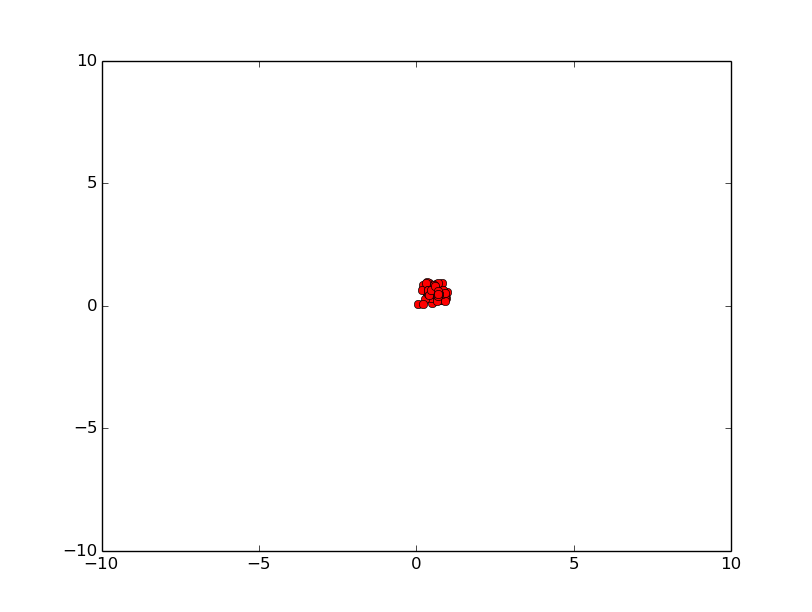
\includegraphics[width=0.45\textwidth]{images/coordinates_start.png} \label{fig:firstbox}}
  \subfloat[]{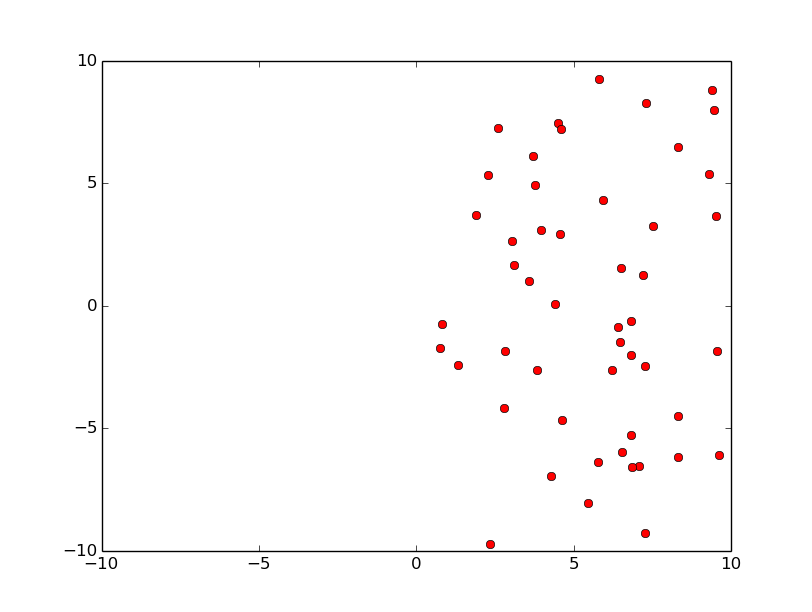
\includegraphics[width=0.45\textwidth]{images/coordinates_start_2.png} \label{fig:secondbox}}
  \caption{
    Pyplot plot of particles in 2 dimensions confined in a box, spanning $x, y \in [0,1]$ for (a) and $x \in [0,10]$ and $y \in [-10,10]$ for (b).
  }
\end{figure}

\newpage

When you have corrected the particle positions, it is time to give the particles random velocities to allow the particles to move around.

\begin{enumerate}[resume]
    \item Create two new lists, \code{velocities\_x} and \code{velocities\_y}, which we shall use to store the velocities for the particles.
    The velocities should be a random number between -10 and 10.
\end{enumerate}

If you want to visualize the velocity vectors for each particle you can use the following function.\\

\begin{lstlisting}
plt.quiver(positions_x, positions_y, velocities_x, velocities_y)
\end{lstlisting}

We are now ready to loop over each particle in our system, but before we do this, you should make it really clear to yourself how we can obtain the coordinates and velocities for the $i$'th particle.

\begin{enumerate}[resume]
  \item How do we access the value of the $i$'th element in the \code{positions\_x} list?
      {\em Hint;} check out task \ref{list operations} from part 1 again.

\end{enumerate}

In this weeks simulation there are no forces that acts on the particles, and only their initial velocities influence their positions.
Hence the location of the $i$'th particle at time $n+1$ can be calculated coordinates and the velocity of the
particle at time $n$, the current time.
\begin{align}
  x_i^{(n+1)} = x^n_i + v_{i}^n \cdot dt
\end{align}

That is, the $i$'th particle will be at its previous position plus its velocity $v_i$ times a time step $dt$.

\begin{enumerate}[resume]
  \item
    Modify your script to loop over each particle and update the $x$- and $y$-coordinates with the respective particle velocities.
    Plot the particle positions after you have changed them to a file called stepcoords.png.
    Does the particles appear to have have moved?

  \item Modify your code to repeat the displacement of the particles \code{n\_step} times.
      Remember to update the positions for each step.

  \item Where are the particles after 10 steps? 100 steps? 1000 steps? 10000 steps?

\end{enumerate}

What you simulate is how particles in vacuum behave if they can not feel each other and have kinetic energy.\\

\newpage

Now we would like to visualize the simulation we have made, because it is a bit hard to see if the simulation has been implemented correctly by just looking at a few images.
What we would like to do is to save a video of what we have done.
To make things easy (as any good cooking show), we have prepared a method for you.\\

On the course website, there is a 'md\_video.py' file.
Save this file, and put it in the same folder as the simulation file.
The function is implemented as following;

\begin{lstlisting}
import md_video as video

...

for n in range(n_steps):

    ...

    # Save a frame every 10 steps
    if n % 10 == 0:
        video.add_frame(positions_x, positions_y)

...

video.save('week1_video')

\end{lstlisting}

where the import statement should be positioned in the head of the file.
A video will be created called \code{week1\_video.mp4}

\begin{enumerate}
  \setcounter{enumi}{7}
  \item Run the simulation from task 9 for \code{n\_steps} = 5000 and save a video.
    Is the video of the simulation as you expect?

\end{enumerate}

What remains is to keep the particles inside a box, i.e. they should make an elastic reflection on the walls and change direction. \\

To change the direction on the $i$'th particle, we must change the sign of the velocity for that particle.
For simplicity, we shall add a box which corresponds to the region we are plotting, that is $x \in [-10,10]$ and $y \in [-10,10]$.
We start out with the $x$-coordinates and then, when we have confirmed that it is working, we move on to the $y$-coordinates.

\begin{enumerate}
  \setcounter{enumi}{8}
  \item Modify your code to check if the updated position of particle $i$ would violate $x \in [-10,10]$.
      If the particle is outside this boundary, change the sign of the $x$-velocity of that
      particular particle before the displacement is made.
      {\em Hint}; you will need if-statements to solve this problem. Also, it is a good idea to draw your plan for what happens with a pen and paper.

  \item Repeat for the $y$-direction.

\end{enumerate}

Is the simulation running as it should be?

% ***************************************************
% END DOCUMENT
% ***************************************************

\end{document}

